
\begin{frame}
  \setbeamercovered{}
  \frametitle{Summary: Experimental Design Overview}
  \begin{adjustwidth}{-15pt}{-10pt}
  \textbf{Pre-detonation nuclear forensics analysis on SNF}\\
  \vspace{2pt}
  \begin{minipage}{0.38\textwidth}
  \onslide<2->{
    \begin{figure}
      \centering
      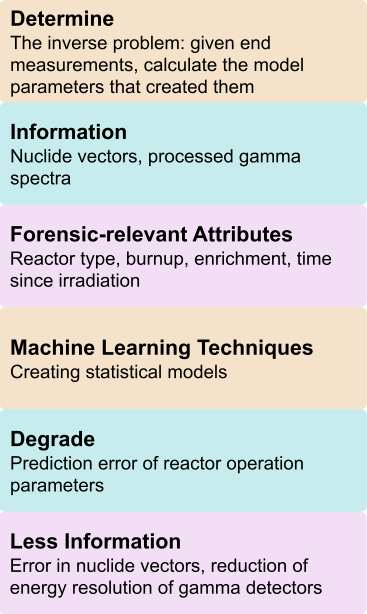
\includegraphics[height=0.78\textheight]{./figures/overview.png}
    \end{figure}
  }
  \end{minipage}%
  \hfill
  \begin{minipage}{0.65\textwidth}
  \onslide<1->{
    \begin{block}{Main Goal:}
      \small
      Is it possible to speed up a nuclear forensics investigation of spent
      nuclear fuel with field-deployable detection?
    \end{block}
  }
    \vspace{-8pt}
  \onslide<3->{
    \begin{block}{Demonstrated:}
      \small
      \begin{itemize}
        \itemsep 0.1em 
        \item Simulation of training data set
        \item Information reduction of training set
        \item Prediction of reactor type, burnup, enrichment, and time since irradiation via:
          \begin{itemize}
            \item \textit{k}-Nearest Neighbors
            \item Decision Trees
            \item Maximum Log-Likelihood Calculations
          \end{itemize}
        \item Evaluation of predictions with respect to information reduction
      \end{itemize}
    \end{block}
  }
  \end{minipage}
  \end{adjustwidth}
\end{frame}

\begin{frame}
  \setbeamercovered{}
  \frametitle{Conclusions}
  \begin{itemize}
    \onslide<1->{
    \item Experiment 1: Nuclide Masses
      \begin{itemize}
        \item Difficult to judge performance baseline, chose generous "standard" from nuclide mass results
        \item SFCOMPO is challenging with this methodology but improvements can be made
      \end{itemize}
    }
    \onslide<2->{
    \item Experiment 2: Processed Gamma Spectra
      \begin{itemize}
        \item Burnup is the only parameter to be well-predicted with gamma spectra
        \item ${}^{235}\text{U}$ enrichment is the only parameter to have very poor performance with gamma spectra
      \end{itemize}
    }
  \end{itemize}
  \vspace{2mm}
  \onslide<3->{
  \hrule
  \vspace{1mm}
  \begin{center}
    Is gamma detection worthy of SNF attribution using this approach? \\ \Large Maybe!
  \end{center}
  }
\end{frame}

\begin{frame}
  \frametitle{Future Work}
  \begin{itemize}
    \item Based on simplifications in this work
      \begin{itemize}
        \item Simulation fidelity (ORIGEN-ARP, homogenized core)
        \item Deeper study on gamma spectra processing
        \item Deeper inquiry into feature reduction
      \end{itemize}
    \item Based on questions this work raised
      \begin{itemize}
        \item Serial prediction, with detailed classification accuracy study 
        \item SFCOMPO improvements, novel imputation approach
        \item Could other statistical methods perform better? Would MLL with $k>1$ perform better?
      \end{itemize}
    \end{itemize}
\end{frame}

